\chapter{TRIỂN KHAI}

\section{Môi trường triển khai và cấu trúc mã nguồn}

Mã nguồn được tổ chức theo cấu trúc của Remix. Thư mục app chứa root, entry.client, entry.server, các route giao diện, route xử lý API, server auth và server database. Cấu trúc này cho phép trình bày rõ từng phần triển khai theo chức năng nghiệp vụ thay vì chỉ mô tả công nghệ chung.


File root.jsx thiết lập Layout, NextUIProvider, import CSS, cấu hình font, nạp Google Translate và nhúng chatbot toàn cục. entry.client.jsx thực hiện hydrate giao diện trên trình duyệt; entry.server.jsx xử lý render phía server. db.server.js khởi tạo PrismaClient; auth.server.js cấu hình session và Auth0Strategy.


\begingroup
\setlength{\tabcolsep}{3pt}
\renewcommand{\arraystretch}{1.25}
\begin{longtable}{|P{0.220\textwidth}|P{0.330\textwidth}|P{0.370\textwidth}|}
\caption{Nhóm file nền tảng của project}\\
\hline
\textbf{File} & \textbf{Vai trò triển khai} & \textbf{Ghi chú} \\
\hline
\endfirsthead
\caption[]{Nhóm file nền tảng của project (tiếp theo)}\\
\hline
\textbf{File} & \textbf{Vai trò triển khai} & \textbf{Ghi chú} \\
\hline
\endhead
root.jsx & Khung layout, provider, CSS và chatbot toàn cục. & Có tích hợp nút dịch ngôn ngữ và component chatbot. \\
\hline
entry.client.jsx & Hydrate RemixBrowser phía client. & Dùng hydrateRoot và StrictMode. \\
\hline
entry.server.jsx & Render HTML phía server. & Dùng renderToPipeableStream, phân biệt bot và browser. \\
\hline
db.server.js & Khởi tạo PrismaClient. & Dùng singleton trong môi trường development. \\
\hline
auth.server.js & Cấu hình cookie session và Auth0. & Cần chuyển secret/callback theo môi trường khi deploy. \\
\hline
\end{longtable}
\endgroup

\section{Thu nhận và xử lý dữ liệu bài tập}

Dữ liệu bài tập được đưa vào hệ thống thông qua quá trình nạp và chuẩn hóa. Các file login.jsx, loader.jsx và saveExercises.jsx cho thấy hệ thống có cơ chế lưu bài tập vào cơ sở dữ liệu bằng Prisma upsert, đồng thời bổ sung các trường tính toán như độ khó, thời lượng, cường độ và nhóm sức khỏe phù hợp.


Việc bổ sung các trường này là cần thiết vì dữ liệu thô thường chưa đủ để phục vụ cá nhân hóa. Nếu một bài tập chỉ có tên và mô tả, hệ thống không thể lọc theo thể trạng hoặc thiết bị. Sau khi xử lý, mỗi bài tập có thể tham gia vào các truy vấn gợi ý và thống kê.



\begin{figure}[H]
    \centering
    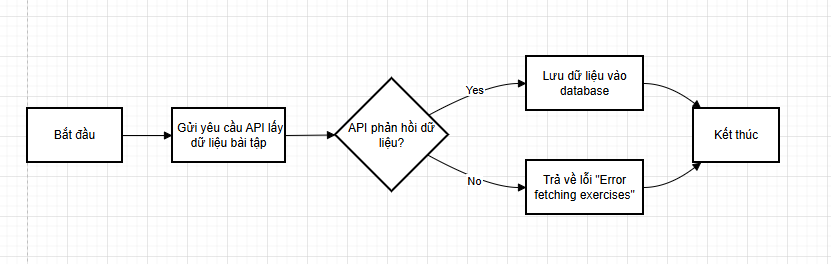
\includegraphics[width=0.86\textwidth,height=0.62\textheight,keepaspectratio]{tai_nguyen/media/image27.png}
    \caption{Quy trình thu nhận dữ liệu bài tập}
\end{figure}

\subsection{Xác định độ khó bài tập}

Hàm calculateDifficulty phân loại bài tập dựa trên thiết bị và bộ phận cơ thể. Các thiết bị nặng như barbell, kettlebell, smith machine hoặc trap bar thường được xếp mức hard. Thiết bị trung bình như dumbbell, resistance band, medicine ball hoặc stability ball được xếp medium. Các bài body weight hoặc thiết bị nhẹ có thể được xếp easy. Nếu thiết bị chưa đủ căn cứ, hệ thống xét tiếp bodyPart để điều chỉnh.



\begin{figure}[H]
    \centering
    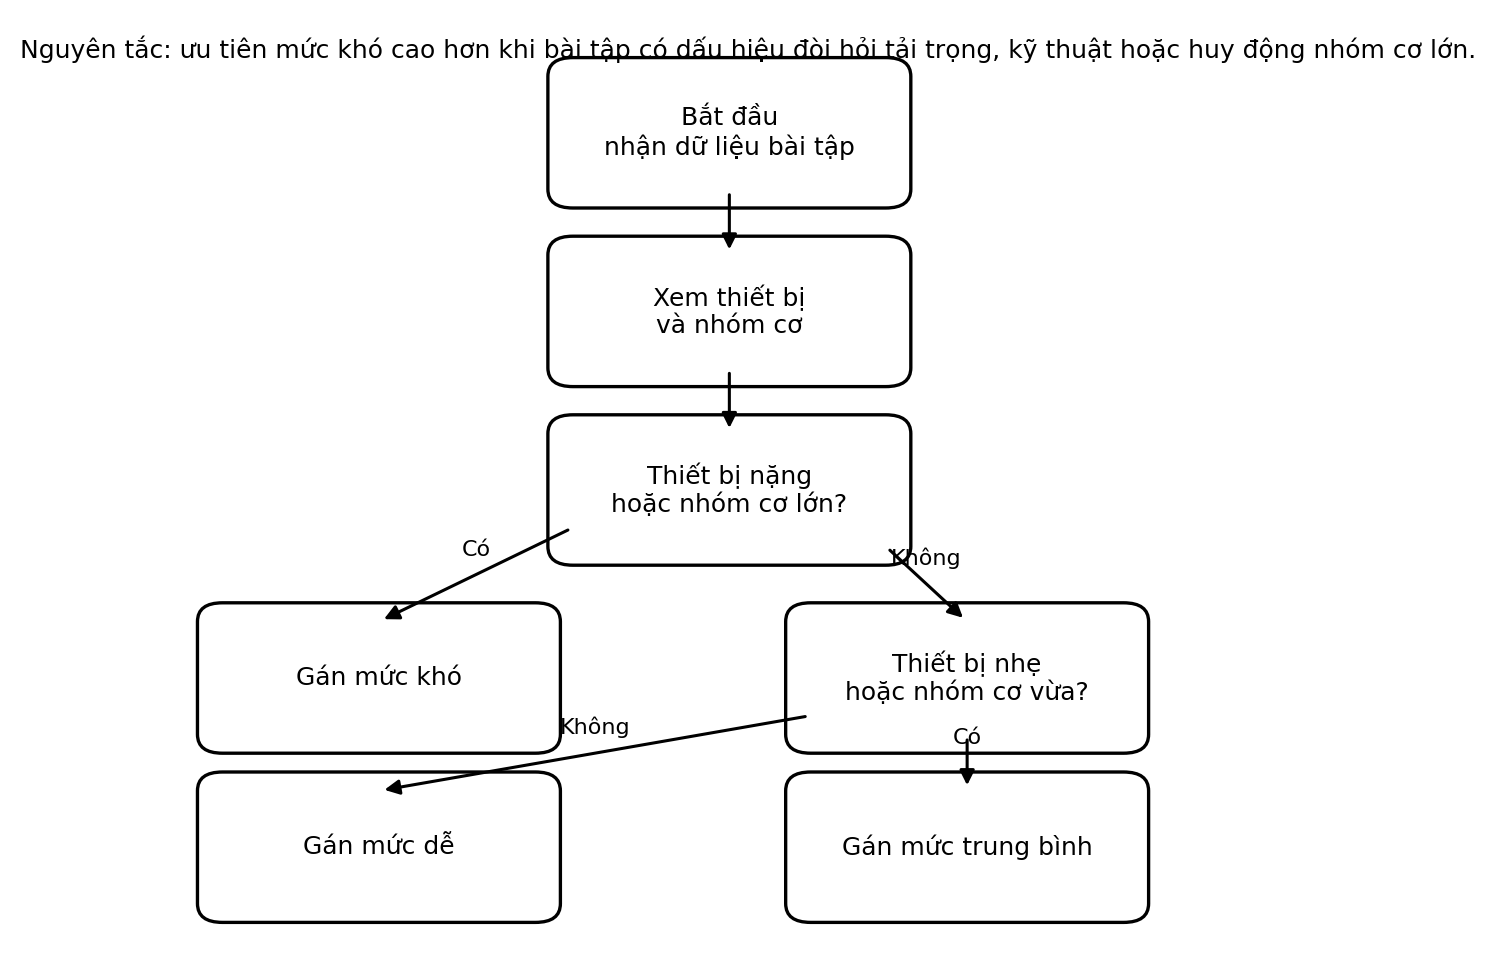
\includegraphics[width=0.86\textwidth,height=0.62\textheight,keepaspectratio]{tai_nguyen/media/image28.png}
    \caption{Quy tắc xác định độ khó bài tập}
\end{figure}

\subsection{Ước lượng thời lượng bài tập}

Hàm calculateTime bắt đầu từ thời gian cơ bản, sau đó cộng hoặc trừ theo thiết bị, nhóm cơ và độ khó. Bài tập dùng thiết bị nặng, tác động nhóm cơ lớn hoặc có độ khó cao sẽ có thời lượng ước lượng lớn hơn. Cách tính này không thay thế giáo án chuyên nghiệp nhưng đủ để hệ thống có trường time phục vụ lọc và hiển thị.



\begin{figure}[H]
    \centering
    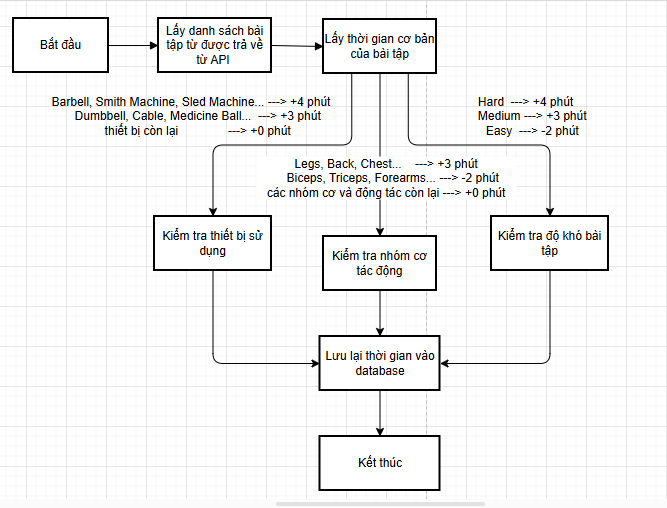
\includegraphics[width=0.86\textwidth,height=0.62\textheight,keepaspectratio]{tai_nguyen/media/image29.png}
    \caption{Quy tắc ước lượng thời lượng bài tập}
\end{figure}

\subsection{Phân loại cường độ}

Hàm calculateIntensity ánh xạ bài tập thành ba mức low, moderate và high. Những bài dùng thiết bị nặng hoặc tác động nhóm cơ lớn thường được xếp high; bài dùng dumbbell, cable, medicine ball hoặc tác động vai, tay được xếp moderate; các trường hợp còn lại mặc định low. Trường intensity là điều kiện quan trọng khi người dùng chọn cường độ mong muốn.



\begin{figure}[H]
    \centering
    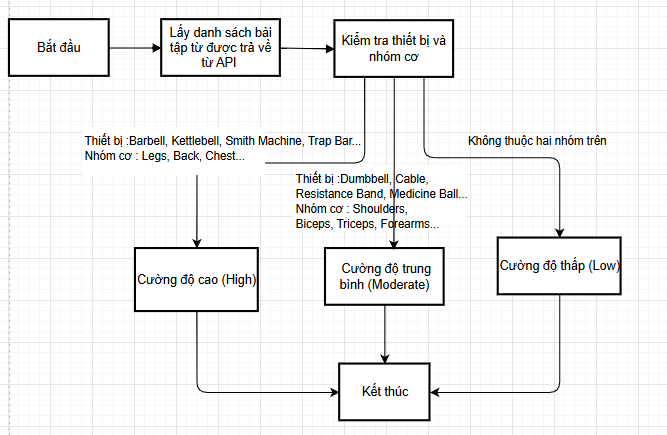
\includegraphics[width=0.86\textwidth,height=0.62\textheight,keepaspectratio]{tai_nguyen/media/image30.png}
    \caption{Quy tắc phân loại cường độ vận động}
\end{figure}

\subsection{Ánh xạ tình trạng sức khỏe}

Hàm calculateHealthConditions gắn bài tập với nhóm sức khỏe. Bài cường độ cao chỉ phù hợp với very healthy; bài moderate phù hợp với normal health và very healthy; bài low có thể phù hợp với weak health, normal health và very healthy. Quy tắc này thể hiện nguyên tắc an toàn: người sức khỏe yếu không nên được gợi ý bài quá nặng.



\begin{figure}[H]
    \centering
    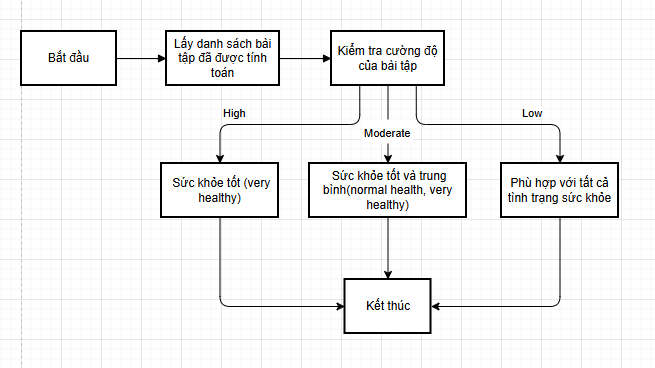
\includegraphics[width=0.86\textwidth,height=0.62\textheight,keepaspectratio]{tai_nguyen/media/image31.png}
    \caption{Quy tắc ánh xạ bài tập với nhóm sức khỏe}
\end{figure}

\section{Triển khai xác thực và quản lý phiên}

Xác thực được triển khai bằng Auth0. Khi người dùng chọn đăng nhập, route auth.auth0.jsx gọi authenticator.authenticate với chiến lược auth0. Sau callback, route homeCallback.jsx điều hướng người dùng về login.jsx. Tại login.jsx, hệ thống kiểm tra email trong cơ sở dữ liệu, tạo user mới nếu chưa có, sau đó lưu userId vào session.


Session được tạo bằng createCookieSessionStorage. Cookie đặt httpOnly để hạn chế truy cập từ JavaScript phía trình duyệt. Trong môi trường production, trường secure cần bật theo biến NODE\_ENV. Cách thiết kế này giúp các route xử lý dữ liệu đọc userId từ session thay vì phụ thuộc dữ liệu gửi từ client.


\section{Triển khai hồ sơ sức khỏe}

Trang HealthStatus.jsx cho phép người dùng nhập các trường sức khỏe và mục tiêu tập luyện. Loader của trang lấy người dùng hiện tại, đọc bản ghi HealthStatus nếu có, đồng thời chuẩn bị danh sách thiết bị và nhóm cơ ban đầu. Khi người dùng thay đổi cường độ, giao diện gọi equipmentapi để lấy danh sách thiết bị phù hợp. Khi chọn thiết bị, giao diện gọi musclesapi để lấy nhóm cơ tương ứng.


healthstatusapi.jsx xử lý lưu dữ liệu. Route này đọc formData, chuyển kiểu số cho cân nặng, chiều cao, tuổi, thời gian rảnh và dùng getUserIdFromSession để xác định chủ sở hữu. Nếu người dùng đã có hồ sơ, hệ thống update; nếu chưa có, hệ thống create. Cách xử lý này bảo đảm mỗi người dùng có thể cập nhật hồ sơ nhiều lần mà không tạo bản ghi trùng.


\section{Triển khai chức năng gợi ý bài tập}

Recommended.workout.jsx là route trọng tâm của chức năng cá nhân hóa. Hàm getRecommendedExercises đọc targetMuscleGroups, equipmentPreference, intensityPreference và condition từ HealthStatus. Sau đó hệ thống truy vấn Exercise với điều kiện AND, loại bỏ các điều kiện rỗng bằng filter(Boolean).


Sau khi nhận danh sách bài tập phù hợp, route xóa các bản ghi Workout cũ của người dùng và tạo danh sách mới. Việc làm mới danh sách giúp dữ liệu gợi ý luôn phản ánh hồ sơ sức khỏe hiện tại. Khi người dùng thay đổi cường độ, thiết bị hoặc nhóm cơ, kết quả gợi ý ở lần mở sau sẽ được tính lại.


\begingroup
\setlength{\tabcolsep}{3pt}
\renewcommand{\arraystretch}{1.25}
\begin{longtable}{|P{0.220\textwidth}|P{0.330\textwidth}|P{0.370\textwidth}|}
\caption{Điều kiện lọc trong chức năng gợi ý}\\
\hline
\textbf{Dữ liệu hồ sơ} & \textbf{Điều kiện truy vấn} & \textbf{Ý nghĩa} \\
\hline
\endfirsthead
\caption[]{Điều kiện lọc trong chức năng gợi ý (tiếp theo)}\\
\hline
\textbf{Dữ liệu hồ sơ} & \textbf{Điều kiện truy vấn} & \textbf{Ý nghĩa} \\
\hline
\endhead
targetMuscleGroups & target in danh sách nhóm cơ & Chỉ lấy bài tác động đúng nhóm cơ người dùng chọn. \\
\hline
equipmentPreference & equipment in danh sách thiết bị & Loại bỏ bài tập yêu cầu thiết bị người dùng không có. \\
\hline
intensityPreference & intensity bằng cường độ đã chọn & Giữ mức vận động phù hợp mong muốn. \\
\hline
condition & healthConditions hasSome condition & Chọn bài có nhóm sức khỏe tương thích. \\
\hline
\end{longtable}
\endgroup

\section{Triển khai lập kế hoạch và lịch tập}

WorkoutPlan.jsx hiển thị danh sách bài tập để người dùng lựa chọn và nhập thông tin kế hoạch như ngày tập, thời gian, số set và số rep. Khi người dùng lưu, dữ liệu selectedExercises được gửi đến Workoutplanapi.jsx.


Workoutplanapi.jsx đọc selectedExercises, lấy userId từ session, sau đó tạo từng bản ghi WorkoutPlan trong cơ sở dữ liệu. Trang Workout.jsx đọc danh sách kế hoạch của người dùng, include thông tin bài tập liên quan và hiển thị theo nhóm ngày. Người dùng có thể sửa thông số bằng editworkoutapi.jsx hoặc xóa kế hoạch bằng deleteapi.jsx.


\section{Triển khai chi tiết bài tập và ghi nhận tiến trình}

ExerciseDetail.jsx và ExerciseDetaill.jsx hiển thị thông tin chi tiết của bài tập, gồm nhóm cơ chính, nhóm cơ phụ, thiết bị, độ khó, ảnh động và hướng dẫn. Trang này có đồng hồ đếm thời gian để người dùng bắt đầu, tạm dừng, đặt lại và lưu thời gian tập.


Khi người dùng nhấn Save, giao diện gửi workoutId, timeSpent và status đến userprogressapi.jsx. Route này kiểm tra userId, kiểm tra bài tập và người dùng có tồn tại, sau đó update hoặc create bản ghi UserProgress. Nhờ vậy, cùng một bài tập có thể được cập nhật tiến trình thay vì tạo nhiều bản ghi không kiểm soát.


\section{Triển khai thống kê và phản hồi cá nhân hóa}

Stats.jsx tổng hợp dữ liệu tiến trình của người dùng và đánh giá theo giai đoạn. Route này đọc userProgress, healthStatus và danh sách bài tập, sau đó tạo các chỉ số phục vụ biểu đồ. Giao diện sử dụng BarChart, PieChart và các thành phần trực quan để người dùng dễ theo dõi.


Hàm generatePersonalizedFeedback tạo phản hồi theo kết quả weekly và monthly. Nếu hiệu suất cần cải thiện, hệ thống khuyến khích tập đều hơn và bắt đầu bằng phiên ngắn. Nếu hiệu suất trung bình, hệ thống gợi ý tăng dần cường độ. Nếu kết quả tốt, hệ thống khuyến khích duy trì và thử thách phù hợp. Ngoài ra, Stats.jsx còn có hàm getRecommendedExercises để đề xuất thêm bài tập dựa trên đánh giá mới.


\section{Triển khai chatbot hỗ trợ}

Chatbot được nhúng thông qua chatbotapi2.jsx. Component tạo cấu hình window.difyChatbotConfig, chèn script embed và thêm CSS để tùy biến nút bong bóng chat, biểu tượng, kích thước cửa sổ và khả năng responsive trên màn hình nhỏ.


Bên cạnh chatbot nhúng, mã nguồn còn có chatbotapi.jsx để lưu tin nhắn vào bảng message với userId, sender và message. Cách này có thể được dùng để mở rộng lịch sử hội thoại nội bộ nếu hệ thống muốn tự quản lý log chat thay vì chỉ dùng nền tảng chatbot bên ngoài.



\begin{figure}[H]
    \centering
    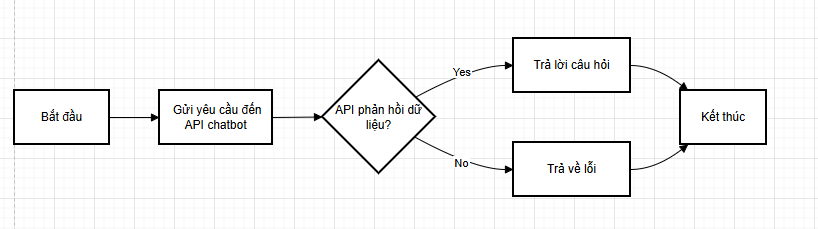
\includegraphics[width=0.86\textwidth,height=0.62\textheight,keepaspectratio]{tai_nguyen/media/image32.png}
    \caption{Luồng tích hợp chatbot vào website}
\end{figure}


\begin{figure}[H]
    \centering
    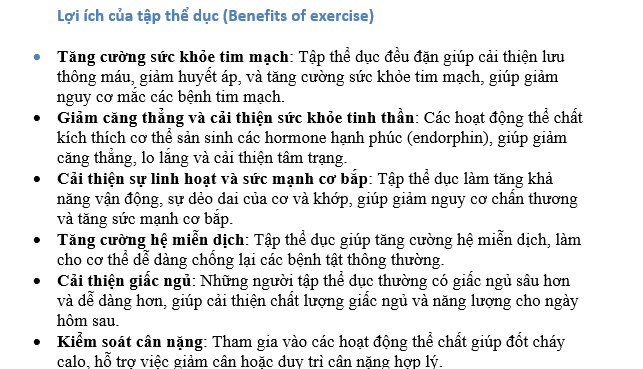
\includegraphics[width=0.86\textwidth,height=0.62\textheight,keepaspectratio]{tai_nguyen/media/image33.png}
    \caption{Bộ dữ liệu câu hỏi dùng cho chatbot}
\end{figure}


\begin{figure}[H]
    \centering
    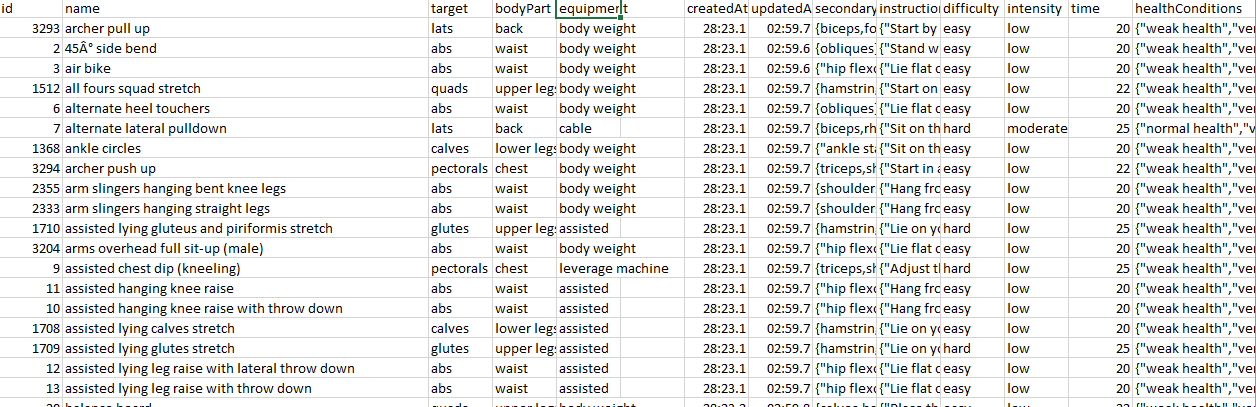
\includegraphics[width=0.86\textwidth,height=0.62\textheight,keepaspectratio]{tai_nguyen/media/image34.png}
    \caption{Bộ dữ liệu bài tập dùng cho chatbot}
\end{figure}


\begin{figure}[H]
    \centering
    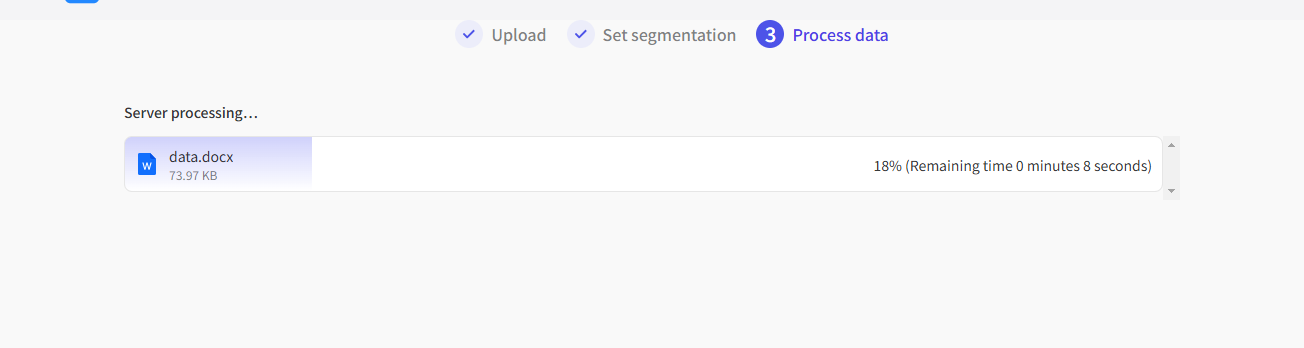
\includegraphics[width=0.86\textwidth,height=0.62\textheight,keepaspectratio]{tai_nguyen/media/image35.png}
    \caption{Quá trình nạp dữ liệu hỏi đáp cho chatbot}
\end{figure}


\begin{figure}[H]
    \centering
    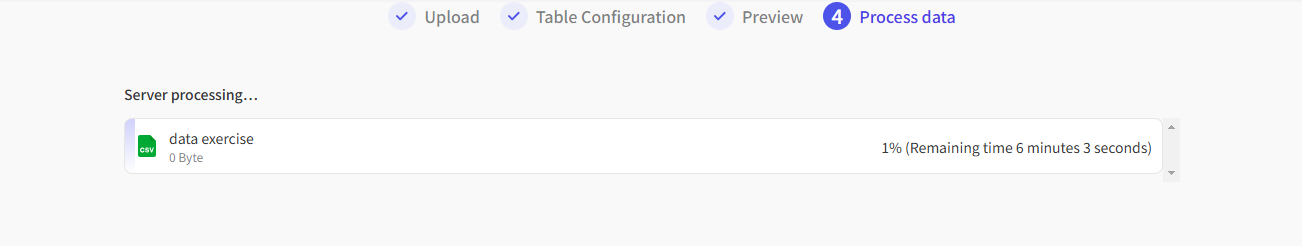
\includegraphics[width=0.86\textwidth,height=0.62\textheight,keepaspectratio]{tai_nguyen/media/image36.png}
    \caption{Quá trình nạp dữ liệu bài tập cho chatbot}
\end{figure}

\section{Triển khai giao diện người dùng}

Các giao diện chính được xây dựng theo luồng sử dụng của người dùng. Phần dưới đây mô tả vai trò của từng màn hình và minh chứng giao diện tương ứng.


Màn hình đăng nhập là điểm bắt đầu của người dùng đã có tài khoản. Từ đây, người dùng được chuyển sang Auth0 để xác thực. Nếu tài khoản hợp lệ, hệ thống điều hướng về trang sau đăng nhập và lưu phiên làm việc.



\begin{figure}[H]
    \centering
    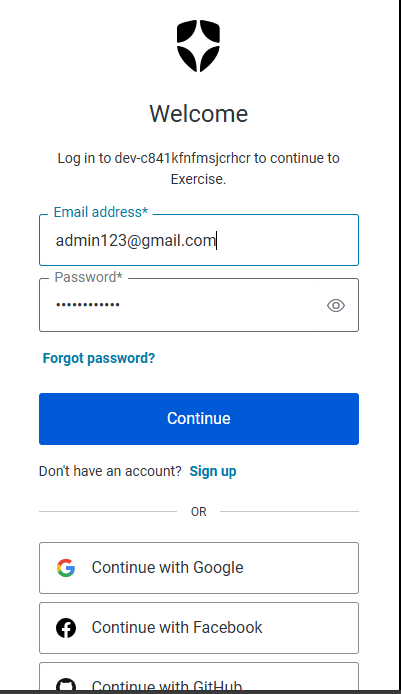
\includegraphics[width=0.86\textwidth,height=0.62\textheight,keepaspectratio]{tai_nguyen/media/image37.png}
    \caption{Giao diện đăng nhập tài khoản}
\end{figure}

Màn hình đăng ký phục vụ người dùng mới. Trong phiên bản dùng Auth0, quá trình tạo tài khoản có thể do Auth0 xử lý, còn website tiếp tục tạo bản ghi User trong cơ sở dữ liệu nội bộ khi đăng nhập thành công lần đầu.



\begin{figure}[H]
    \centering
    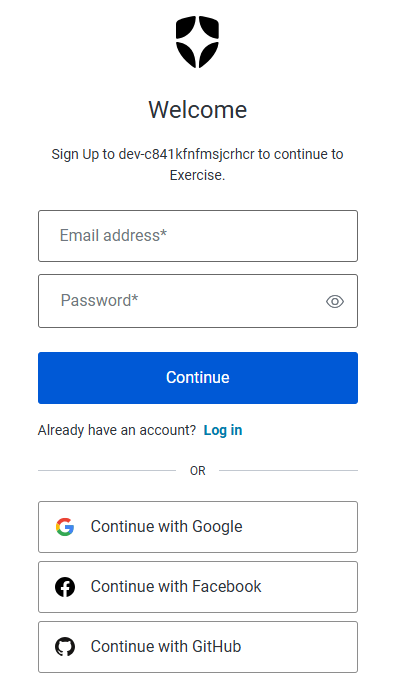
\includegraphics[width=0.86\textwidth,height=0.62\textheight,keepaspectratio]{tai_nguyen/media/image38.png}
    \caption{Giao diện tạo tài khoản mới}
\end{figure}

Trang chủ hiển thị thư viện bài tập, banner, các nhóm nội dung giới thiệu và thanh tìm kiếm. Danh sách bài tập được phân trang để giảm tải giao diện khi dữ liệu lớn.



\begin{figure}[H]
    \centering
    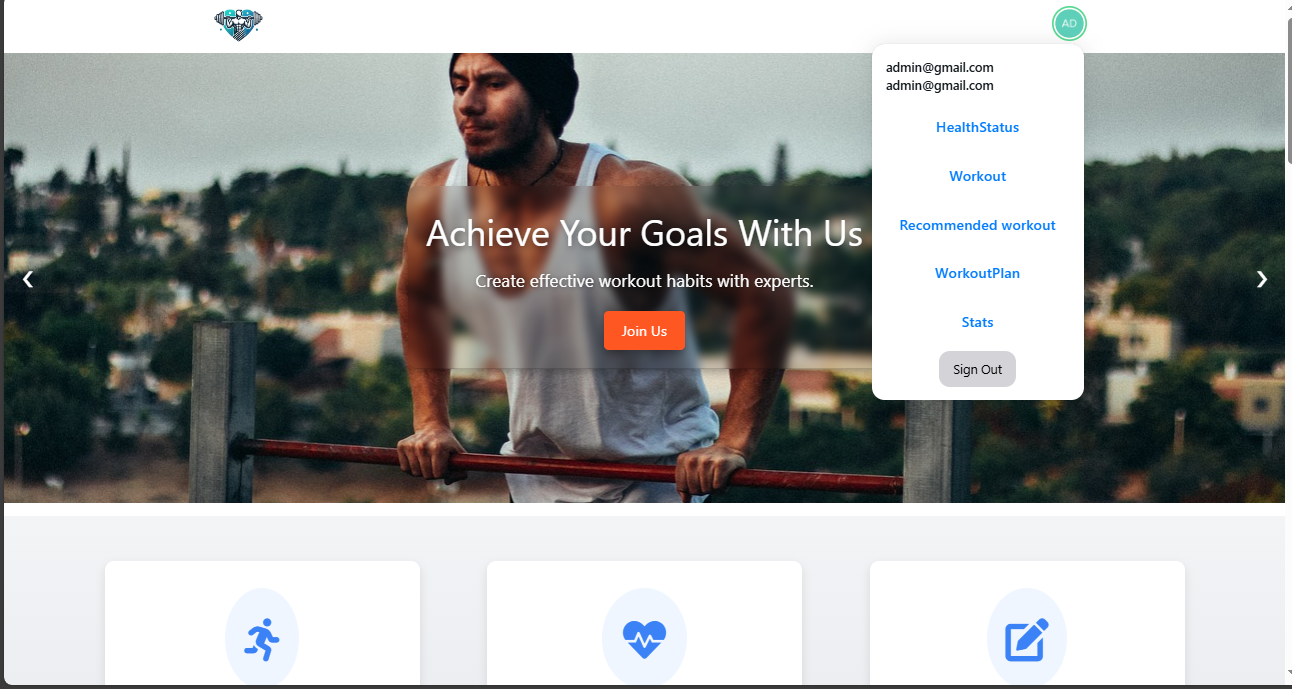
\includegraphics[width=0.86\textwidth,height=0.62\textheight,keepaspectratio]{tai_nguyen/media/image39.png}
    \caption{Giao diện trang chủ sau khi đăng nhập}
\end{figure}

Trang chủ hiển thị thư viện bài tập, banner, các nhóm nội dung giới thiệu và thanh tìm kiếm. Danh sách bài tập được phân trang để giảm tải giao diện khi dữ liệu lớn.



\begin{figure}[H]
    \centering
    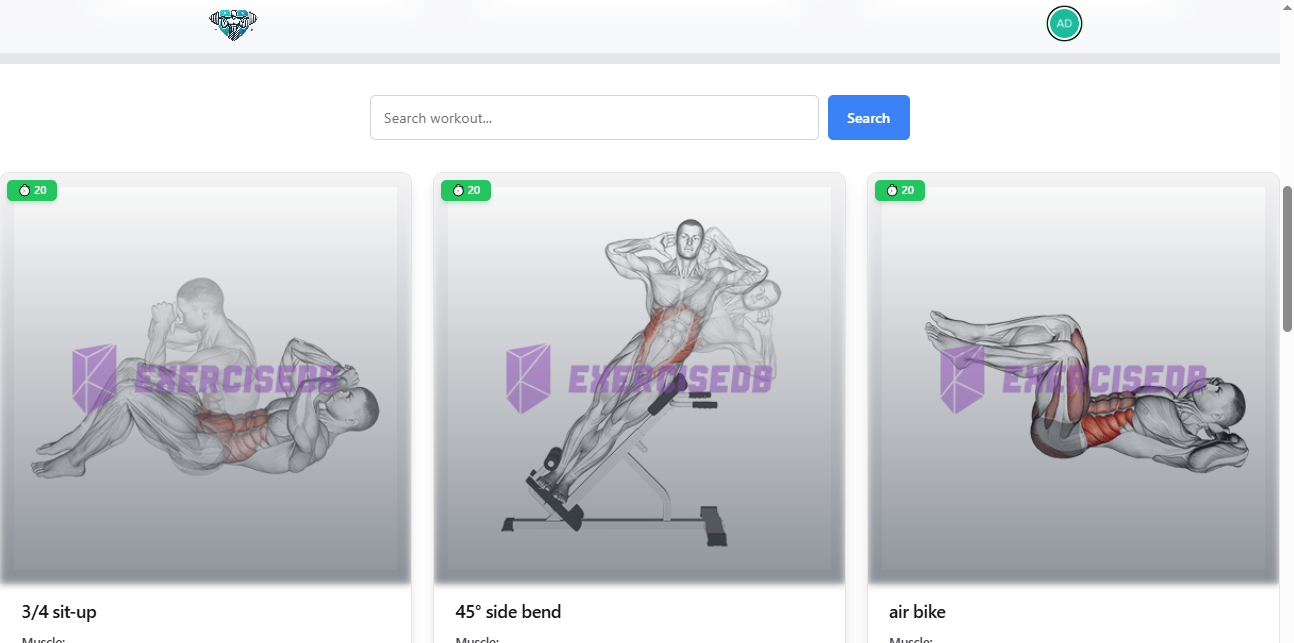
\includegraphics[width=0.86\textwidth,height=0.62\textheight,keepaspectratio]{tai_nguyen/media/image40.png}
    \caption{Bố cục nội dung trang chủ và danh sách bài tập}
\end{figure}

Trang hồ sơ sức khỏe là bước quan trọng trước khi nhận gợi ý. Người dùng khai báo tình trạng, mục tiêu, thiết bị, nhóm cơ và thời gian, từ đó hệ thống có dữ liệu để cá nhân hóa.



\begin{figure}[H]
    \centering
    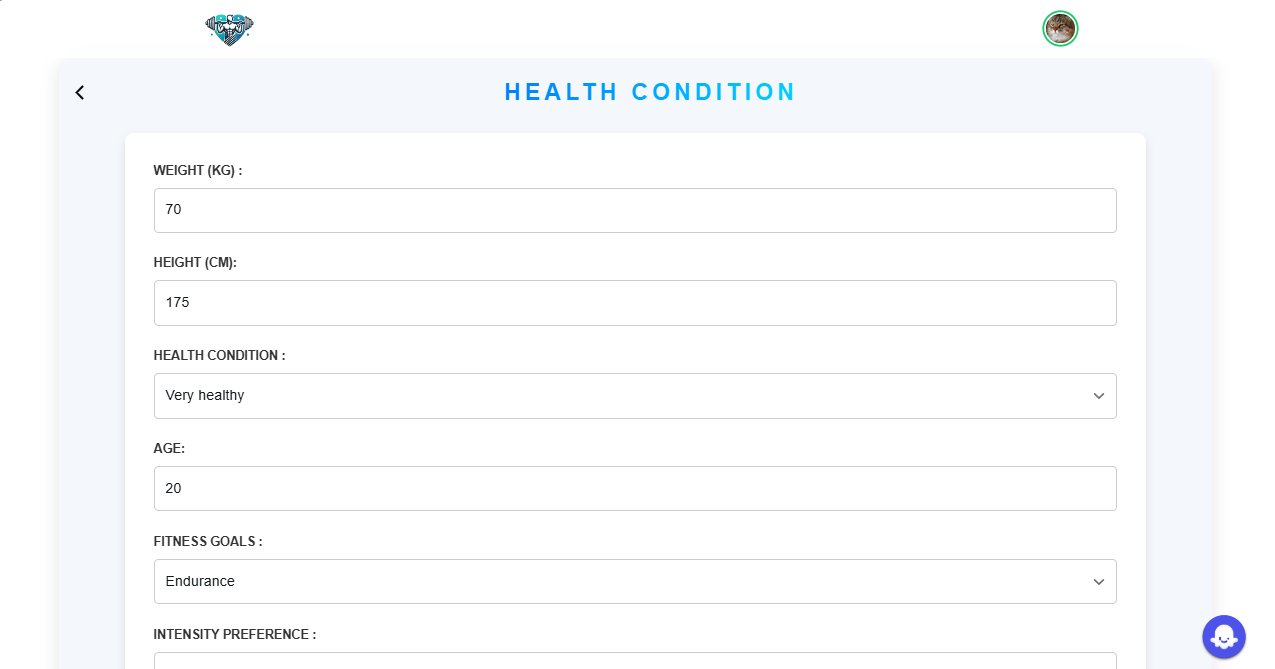
\includegraphics[width=0.86\textwidth,height=0.62\textheight,keepaspectratio]{tai_nguyen/media/image41.png}
    \caption{Giao diện cập nhật hồ sơ sức khỏe}
\end{figure}

Trang bài tập đề xuất hiển thị kết quả sau khi lọc theo hồ sơ sức khỏe. Người dùng có thể xem thông tin cơ bản, hình minh họa và chuyển sang các thao tác tiếp theo.



\begin{figure}[H]
    \centering
    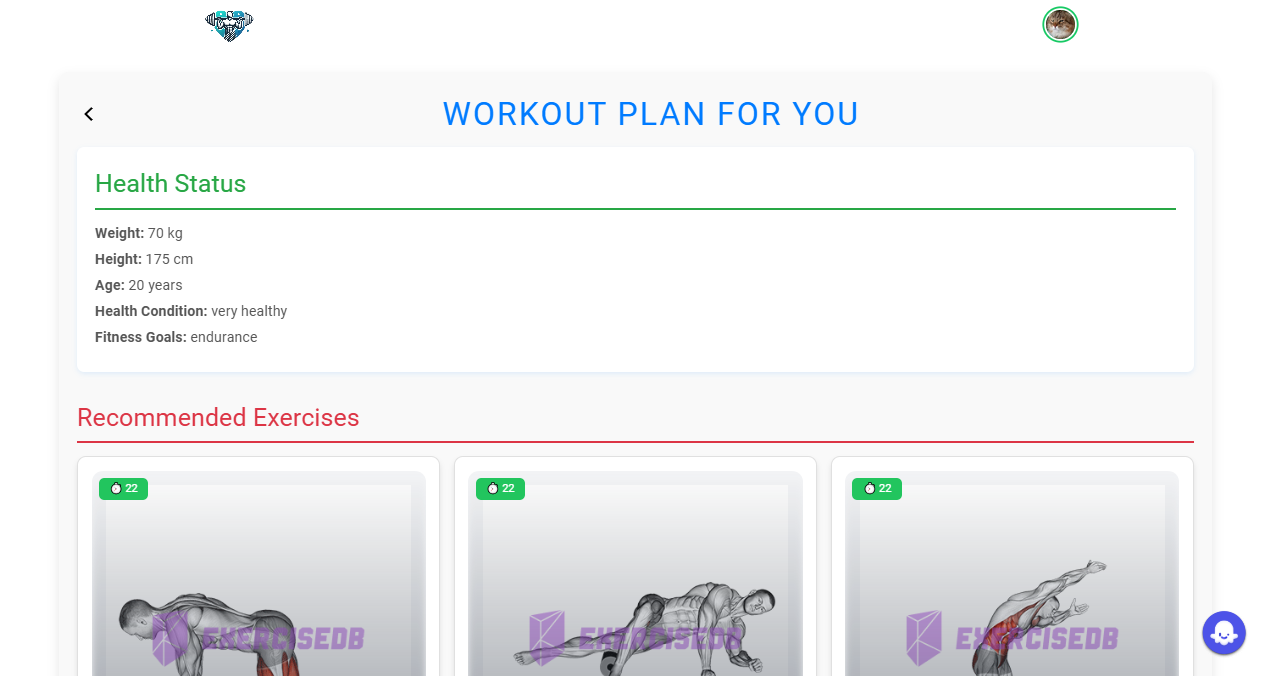
\includegraphics[width=0.86\textwidth,height=0.62\textheight,keepaspectratio]{tai_nguyen/media/image42.png}
    \caption{Giao diện danh sách bài tập đề xuất}
\end{figure}

Trang lập kế hoạch giúp người dùng chọn bài tập và đưa vào lịch cá nhân. Đây là bước chuyển từ gợi ý sang kế hoạch cụ thể có ngày, thời lượng, số hiệp và số lần lặp.



\begin{figure}[H]
    \centering
    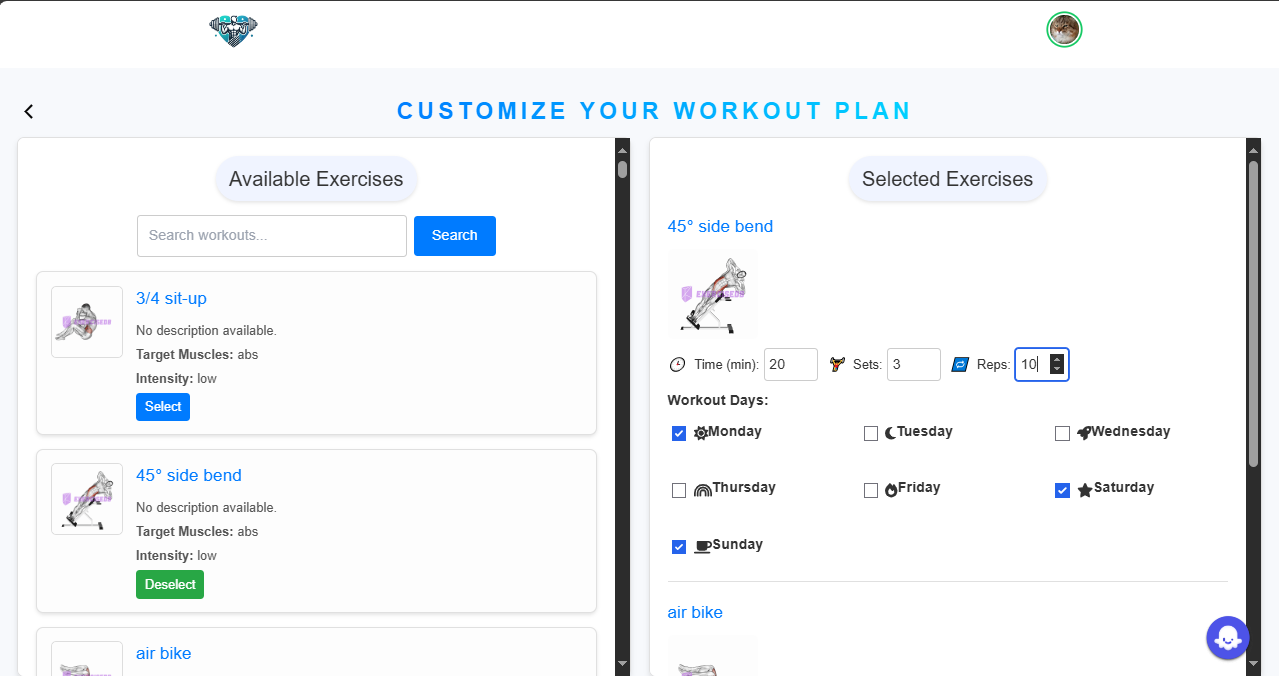
\includegraphics[width=0.86\textwidth,height=0.62\textheight,keepaspectratio]{tai_nguyen/media/image43.png}
    \caption{Giao diện lập kế hoạch tập luyện}
\end{figure}

Trang lịch bài tập cá nhân hiển thị các bài đã được lưu theo ngày. Người dùng có thể chỉnh sửa hoặc xóa bài tập trong kế hoạch nếu lịch thay đổi.



\begin{figure}[H]
    \centering
    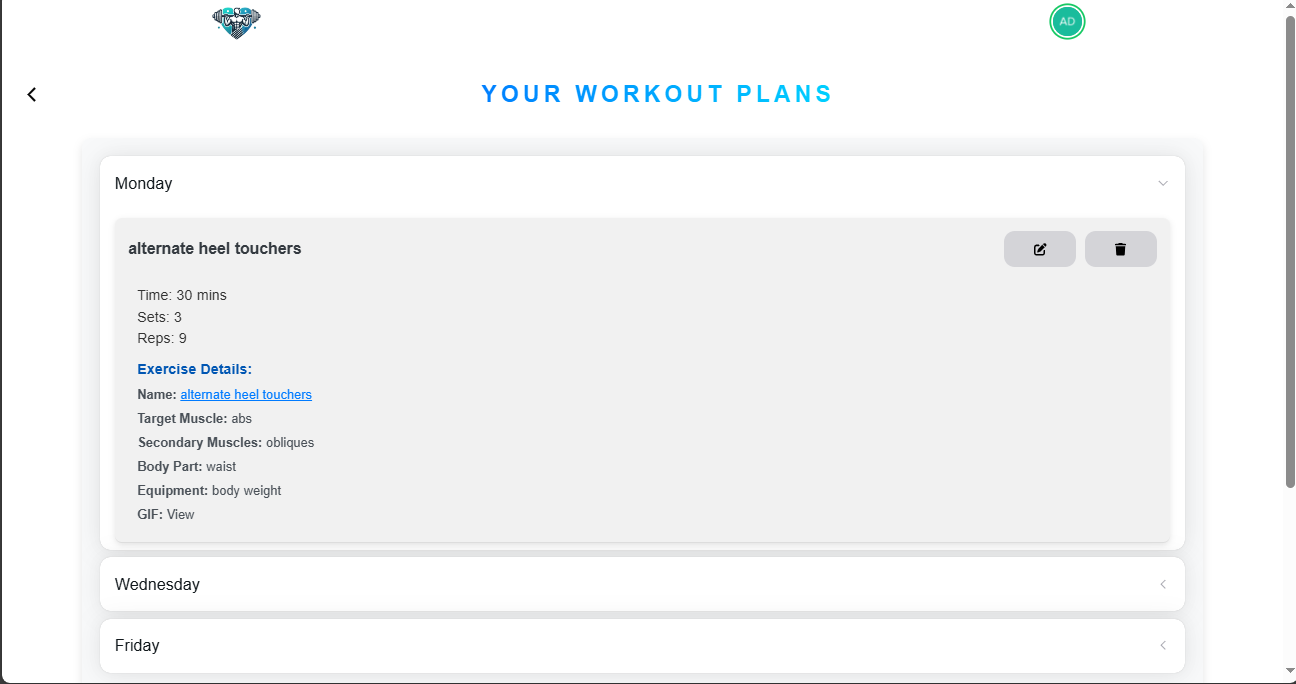
\includegraphics[width=0.86\textwidth,height=0.62\textheight,keepaspectratio]{tai_nguyen/media/image44.png}
    \caption{Giao diện lịch bài tập cá nhân}
\end{figure}

Trang thống kê tổng hợp dữ liệu luyện tập và phản hồi. Biểu đồ giúp người dùng nhận ra tần suất, thời lượng và xu hướng duy trì thói quen.



\begin{figure}[H]
    \centering
    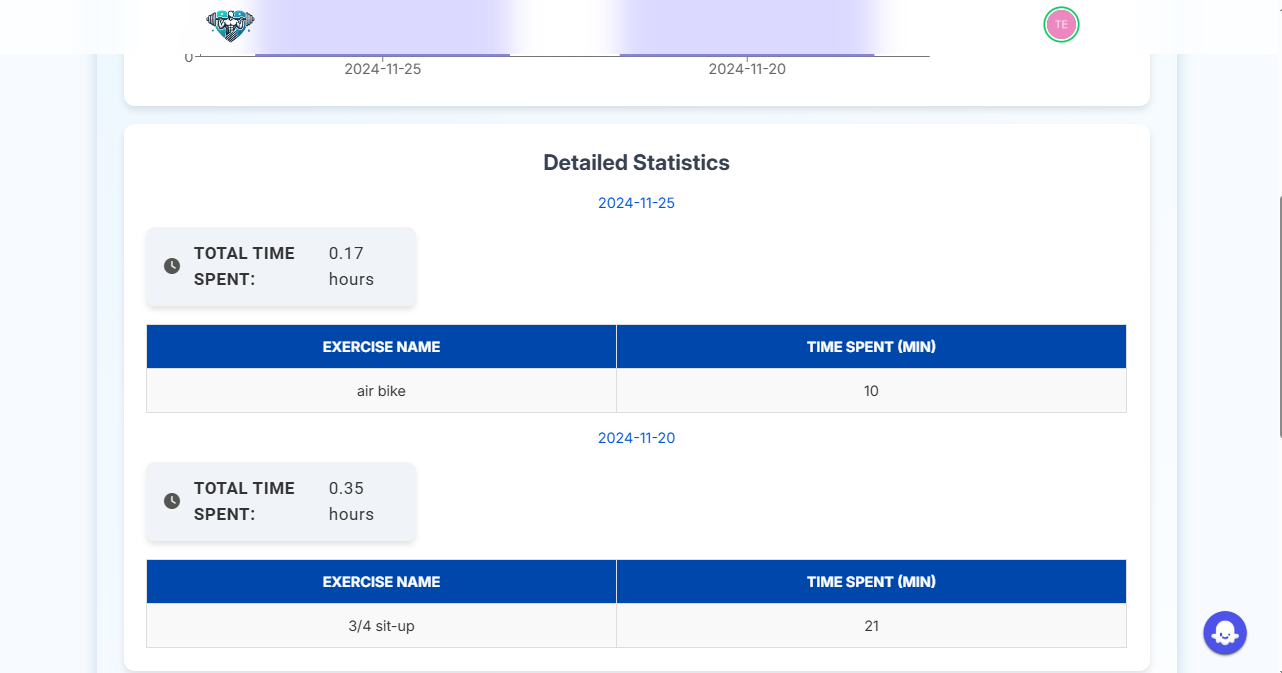
\includegraphics[width=0.86\textwidth,height=0.62\textheight,keepaspectratio]{tai_nguyen/media/image45.png}
    \caption{Giao diện thống kê kết quả tập luyện}
\end{figure}

Cửa sổ chatbot được đặt ở vị trí dễ truy cập nhưng không làm mất chức năng chính của website. Người dùng có thể hỏi nhanh về bài tập hoặc cách sử dụng hệ thống.



\begin{figure}[H]
    \centering
    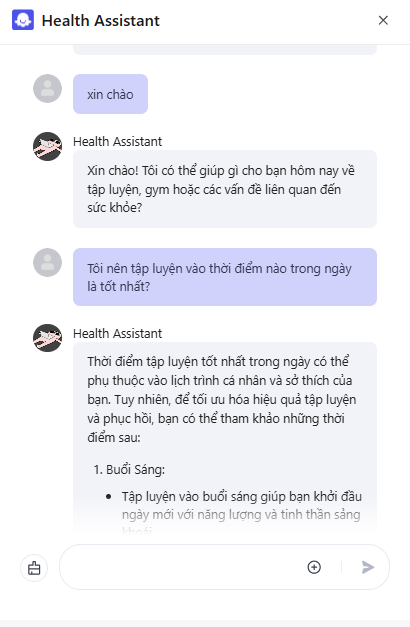
\includegraphics[width=0.86\textwidth,height=0.62\textheight,keepaspectratio]{tai_nguyen/media/image46.png}
    \caption{Giao diện trao đổi với chatbot}
\end{figure}

\section{Triển khai giao diện quản trị}

admin.jsx triển khai dashboard dành cho tài khoản có quyền quản trị. Loader kiểm tra xác thực Auth0, tìm người dùng theo email, kiểm tra cờ isAdmin và chuyển hướng về trang lỗi nếu không đủ quyền. Khi hợp lệ, admin nhận dữ liệu thống kê, danh sách người dùng và danh sách bài tập.


Giao diện quản trị có ba nhóm chính: dashboard tổng quan, quản lý người dùng và quản lý bài tập. Admin có thể sửa email, tên người dùng, quyền admin, xóa tài khoản, thêm bài tập, sửa bài tập hoặc xóa bài tập. Các thao tác này gọi đến các route update\_user, delete\_user, create\_exercise, update\_exercise và delete\_exercise.



\begin{figure}[H]
    \centering
    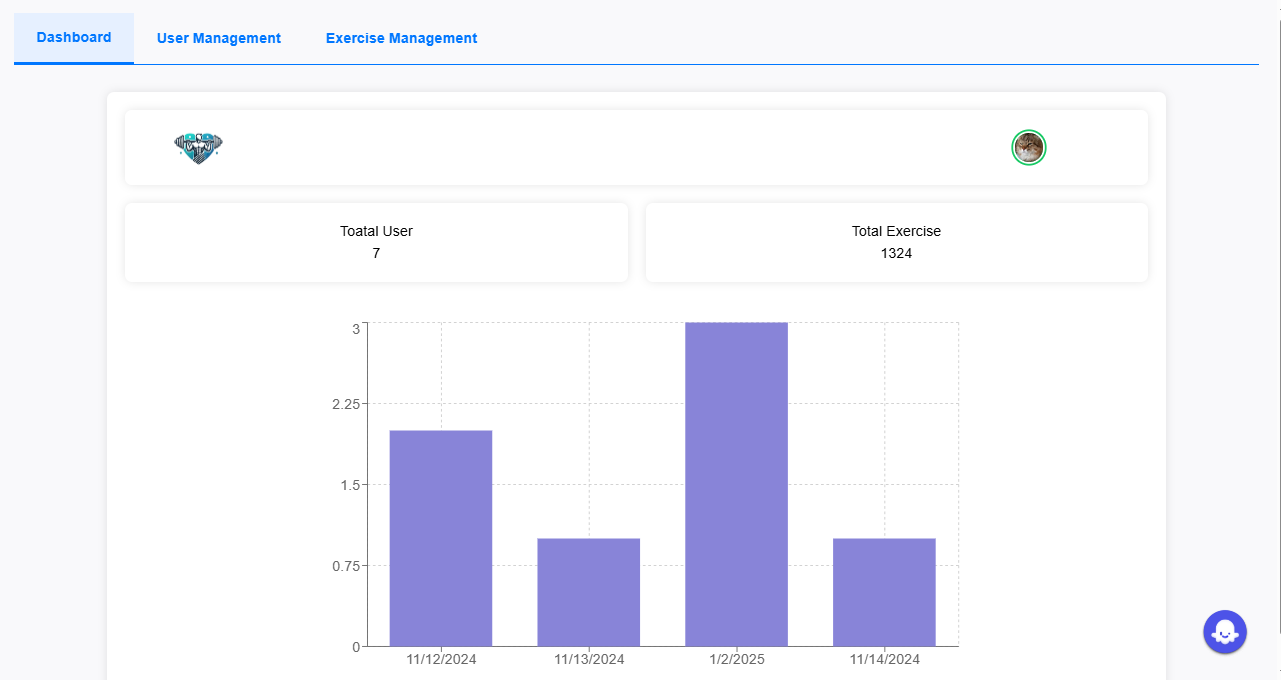
\includegraphics[width=0.86\textwidth,height=0.62\textheight,keepaspectratio]{tai_nguyen/media/image47.png}
    \caption{Giao diện tổng quan dành cho quản trị viên}
\end{figure}


\begin{figure}[H]
    \centering
    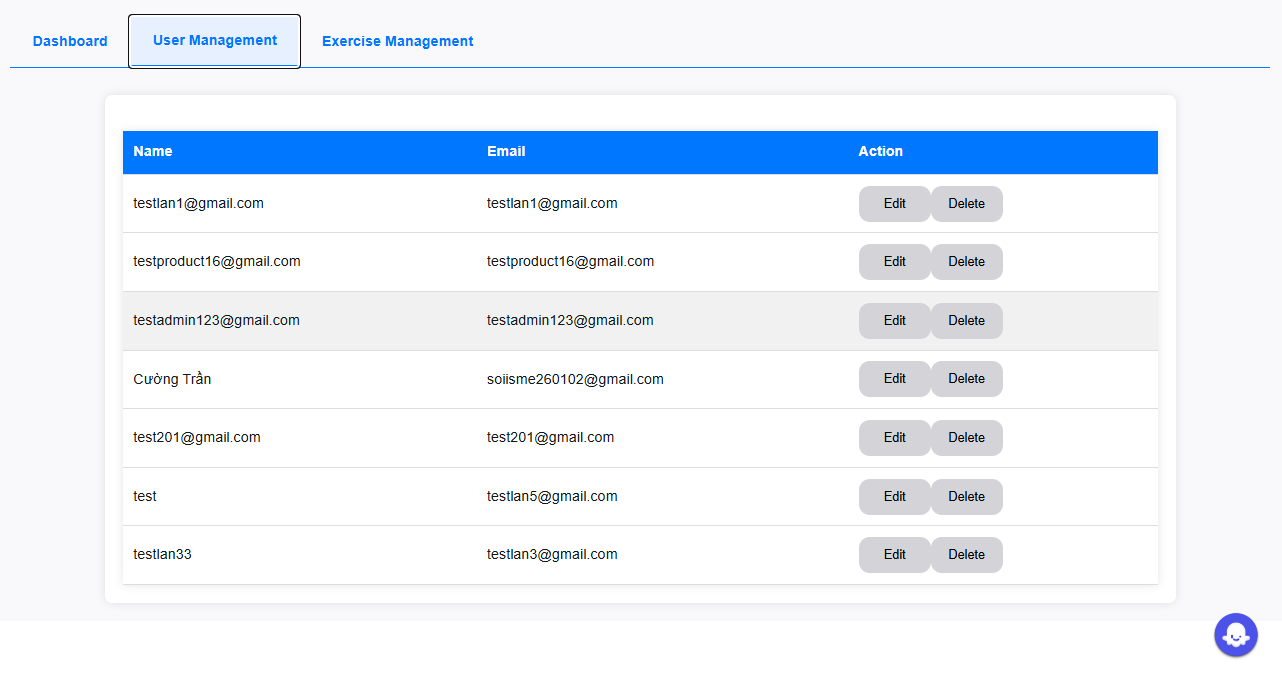
\includegraphics[width=0.86\textwidth,height=0.62\textheight,keepaspectratio]{tai_nguyen/media/image48.png}
    \caption{Giao diện quản lý tài khoản người dùng}
\end{figure}


\begin{figure}[H]
    \centering
    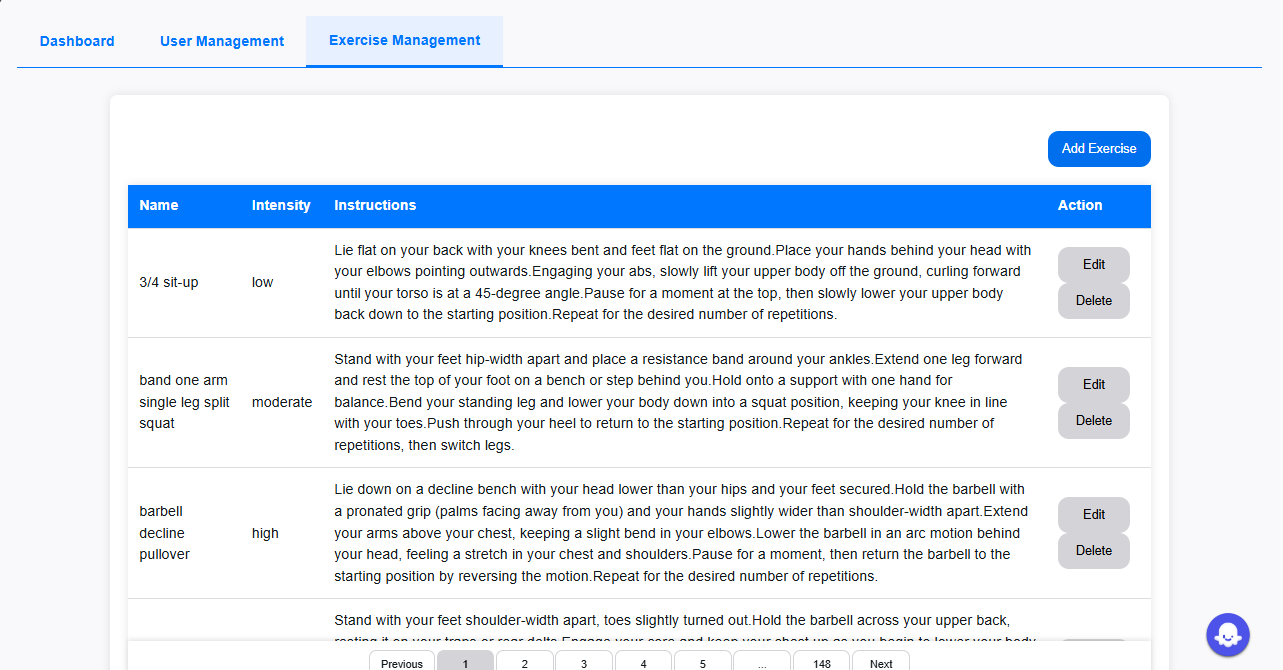
\includegraphics[width=0.86\textwidth,height=0.62\textheight,keepaspectratio]{tai_nguyen/media/image49.png}
    \caption{Giao diện quản lý dữ liệu bài tập}
\end{figure}

\section{Kiểm thử chức năng}

Kiểm thử được thực hiện theo từng luồng nghiệp vụ. Mỗi ca kiểm thử gồm điều kiện đầu vào, thao tác, kết quả mong đợi và trạng thái. Kiểm thử tập trung vào các chức năng có tác động đến dữ liệu như đăng nhập, hồ sơ sức khỏe, gợi ý, lưu kế hoạch, ghi tiến trình, thống kê và quản trị.


\begingroup
\small
\setlength{\tabcolsep}{3pt}
\renewcommand{\arraystretch}{1.25}
\begin{longtable}{|P{0.160\textwidth}|P{0.280\textwidth}|P{0.280\textwidth}|P{0.200\textwidth}|}
\caption{Kịch bản kiểm thử chức năng chính}\\
\hline
\textbf{Mã} & \textbf{Kịch bản} & \textbf{Kết quả mong đợi} & \textbf{Trạng thái} \\
\hline
\endfirsthead
\caption[]{Kịch bản kiểm thử chức năng chính (tiếp theo)}\\
\hline
\textbf{Mã} & \textbf{Kịch bản} & \textbf{Kết quả mong đợi} & \textbf{Trạng thái} \\
\hline
\endhead
TC-01 & Đăng nhập bằng tài khoản hợp lệ & Người dùng được chuyển vào hệ thống và có session userId. & Đạt \\
\hline
TC-02 & Mở trang gợi ý khi chưa có hồ sơ sức khỏe & Hệ thống trả thông báo cần cập nhật hồ sơ. & Đạt \\
\hline
TC-03 & Lưu hồ sơ sức khỏe hợp lệ & Dữ liệu được create hoặc update trong HealthStatus. & Đạt \\
\hline
TC-04 & Nhận bài tập đề xuất & Danh sách bài tập thỏa điều kiện được hiển thị. & Đạt \\
\hline
TC-05 & Lưu kế hoạch tập & WorkoutPlan tạo bản ghi theo userId và bài tập đã chọn. & Đạt \\
\hline
TC-06 & Sửa/xóa kế hoạch & Thông số được cập nhật hoặc bản ghi bị xóa. & Đạt \\
\hline
TC-07 & Lưu tiến trình từ trang chi tiết & UserProgress được tạo hoặc cập nhật. & Đạt \\
\hline
TC-08 & Xem thống kê & Biểu đồ và phản hồi được tạo từ dữ liệu tiến trình. & Đạt \\
\hline
TC-09 & Truy cập admin bằng user thường & Hệ thống chuyển hướng hoặc từ chối quyền truy cập. & Đạt \\
\hline
TC-10 & Admin thêm/sửa/xóa bài tập & Dữ liệu Exercise thay đổi đúng thao tác. & Đạt \\
\hline
\end{longtable}
\endgroup


\begin{figure}[H]
    \centering
    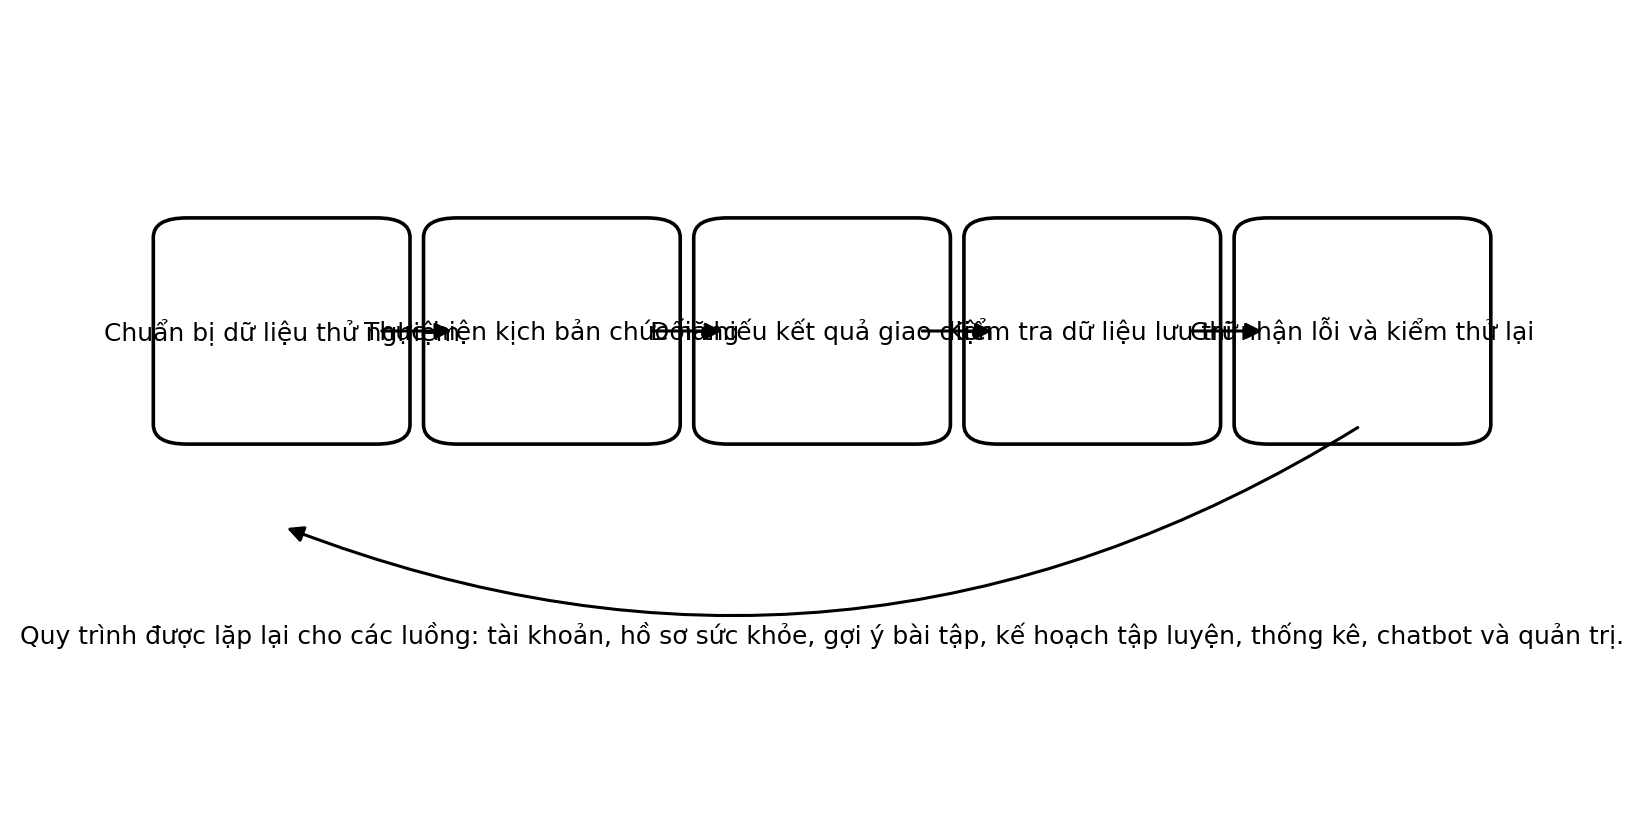
\includegraphics[width=0.86\textwidth,height=0.62\textheight,keepaspectratio]{tai_nguyen/media/image50.png}
    \caption{Quy trình kiểm thử các luồng chức năng}
\end{figure}

\section{Đánh giá bảo mật khi triển khai}

Ở mức sản phẩm thử nghiệm, hệ thống đã có xác thực Auth0 và kiểm tra session cho các route cần dữ liệu cá nhân. Tuy nhiên, khi triển khai thật cần rà soát toàn bộ secret, API key, token chatbot và khóa RapidAPI. Những giá trị này phải đặt trong biến môi trường hoặc hệ thống quản lý secret, không lưu trực tiếp trong mã nguồn.


Một số route quản trị đã kiểm tra quyền ở loader của trang admin. Tuy vậy, để an toàn hơn, các action quản trị cũng nên kiểm tra lại quyền admin trước khi thực hiện create, update hoặc delete. Đây là lớp bảo vệ cần thiết vì người dùng có thể gửi request trực tiếp mà không thông qua giao diện.


Dữ liệu sức khỏe là dữ liệu nhạy cảm ở mức cá nhân. Vì vậy, hệ thống cần giới hạn hiển thị theo userId, không cho user xem hồ sơ của người khác và chỉ đưa thông tin tối thiểu vào chatbot.


\section{Đánh giá kết quả triển khai}

\begingroup
\setlength{\tabcolsep}{3pt}
\renewcommand{\arraystretch}{1.25}
\begin{longtable}{|P{0.220\textwidth}|P{0.330\textwidth}|P{0.370\textwidth}|}
\caption{Đối chiếu kết quả triển khai với mục tiêu}\\
\hline
\textbf{Mục tiêu} & \textbf{Kết quả đạt được} & \textbf{Nhận xét} \\
\hline
\endfirsthead
\caption[]{Đối chiếu kết quả triển khai với mục tiêu (tiếp theo)}\\
\hline
\textbf{Mục tiêu} & \textbf{Kết quả đạt được} & \textbf{Nhận xét} \\
\hline
\endhead
Xác thực tài khoản & Đã cấu hình Auth0, session và tạo User nội bộ. & Đáp ứng chức năng nền tảng. \\
\hline
Hồ sơ sức khỏe & Đã có form nhập và API lưu/cập nhật. & Phục vụ trực tiếp cho gợi ý. \\
\hline
Thư viện bài tập & Đã có danh sách, tìm kiếm, phân trang và chi tiết. & Có thể mở rộng thêm bộ lọc. \\
\hline
Gợi ý cá nhân hóa & Đã lọc theo nhóm cơ, thiết bị, cường độ và sức khỏe. & Phù hợp với phạm vi rule-based. \\
\hline
Kế hoạch tập & Đã lưu, xem, sửa và xóa kế hoạch. & Đáp ứng nhu cầu theo dõi lịch. \\
\hline
Tiến trình và thống kê & Đã ghi nhận thời gian, trạng thái và tạo phản hồi. & Cần bổ sung thêm chỉ số nếu triển khai thực tế. \\
\hline
Chatbot & Đã nhúng trợ lý hội thoại vào giao diện. & Cần tiếp tục kiểm soát nội dung trả lời. \\
\hline
Quản trị & Đã có dashboard, quản lý user và bài tập. & Cần tăng kiểm tra quyền ở action. \\
\hline
\end{longtable}
\endgroup

\section{Hướng dẫn vận hành và bảo trì}

\begin{itemize}

    \item Khi chạy hệ thống ở môi trường phát triển, cần cấu hình các biến môi trường cho Auth0, session secret, database URL và các dịch vụ ngoài. Sau đó chạy migration Prisma nếu có schema, nạp dữ liệu bài tập ban đầu và kiểm tra tài khoản admin.

    \item Khi cập nhật bài tập, admin nên kiểm tra đủ các trường name, target, secondaryMuscles, bodyPart, equipment, gifUrl, difficulty, time, intensity, healthConditions và instructions. Nếu thiếu các trường này, chức năng gợi ý hoặc hiển thị chi tiết có thể bị lỗi.

    \item Khi cập nhật chatbot, cần kiểm tra nội dung huấn luyện, câu trả lời mẫu và giới hạn phạm vi. Các câu hỏi liên quan đến bệnh lý, chấn thương hoặc thuốc nên được trả lời theo hướng khuyến nghị gặp chuyên gia.

\end{itemize}
